\documentclass[english]{article}
\usepackage[T1]{fontenc}
\usepackage[utf8]{inputenc}
\usepackage{babel}
\usepackage[unicode=true,pdfusetitle,
 bookmarks=true,bookmarksnumbered=false,bookmarksopen=false,
 breaklinks=true,pdfborder={0 0 1},backref=false,colorlinks=false]
 {hyperref}
\usepackage{tabularx}
\usepackage{graphicx}
\graphicspath{{images/}}
\usepackage{svg}
\usepackage{float}
\usepackage{titling}
\renewcommand{\arraystretch}{1.4}
\newcommand{\code}[1]{\texttt{#1}}
\usepackage{array}

\pretitle{%
	\begin{center}
		\LARGE
		
\includegraphics[width=250pt]{../other/Logo_blu.png}\\[\bigskipamount]~\\[\bigskipamount]
	}
\posttitle{\end{center}}

\begin{document}

\title{Politecnico di Milano\\
 A.A. 2016–2017 \\
Software Engineering 2: “PowerEnJoy” \\
\emph{Integration Test Plan Document}}

\author{Pietro Ferretti, Nicole Gervasoni, Danilo Labanca}
\date{January 15, 2017}
\maketitle

\newpage

\tableofcontents{}

\newpage

\section{Introduction}

\subsection{Revision History}
\begin{itemize}
	\item{ITDP v1.0, published on January 15, 2017}
\end{itemize}
\subsection{Purpose and Scope}

\paragraph{}
The purpose of this document is to provide a complete description of the integration testing plans for PowerEnjoy. It will focus on testing the proper behavior of the software by checking the
interoperability between its components.
It is intended for developers and for any team member involved in the testing process.
%TODO inserire outline dei contenuti?

\paragraph{}
The aim of this project is to specify in detail a new digital management software for PowerEnJoy, a car-sharing service that employs electric cars only.

\paragraph{}
PowerEnjoy will offer a very valuable service to its users, letting them borrow cars to drive around the city freely, as an alternative to their own vehicles and public transport.
Among the advantages of using PowerEnJoy we can note begin able to find available cars in any place that is served by our system and having dedicated spots to park in (namely, PowerEnJoy's power grid stations).
Furthermore, thanks to the fact that all the cars that we provide are electrically powered, PowerEnJoy is also very environmentally friendly.

%\paragraph{}
%PowerEnJoy's users, after registering, will be able to reserve, unlock and drive the cars our system will provide. Users will be charged per minute until they park the car in a safe area and end the ride.
%Users will be able to park their car temporarily and use it again later, or end their ride remotely.
%
%Our system will incentivize virtuous behaviour by offering several discounts if certain conditions are met (like charging a car at a power grid station).

\subsection{List of Definitions and Abbreviations}

\subsubsection{Definitions}

\begin{itemize}
\item{\textit{Guest}: a person that is not registered to the system.}
\item{\textit{User}: a person that is registered to the system. Users can log in to the system with their email or username and their password. Their first name, last name, date of birth, driving license ID are stored in the database.}
\item{\textit{Safe area}: a location where the user can park and leave the car. Users can end their ride and park temporarily only in these locations. The set of safe areas is predefined by the system.}
\item{\textit{Power grid station}: a place where cars can be parked and plugged in. While a car is plugged in a power grid station its battery will be recharged. Power grid stations are by definition safe areas.}
\item{\textit{Available car}: a car that is currently not begin used by any user, and has not been reserved either. Available cars are in good conditions (not dirty nor damaged) and don’t have dead batteries.}
\item{\textit{Reservation}:
	\begin{itemize}
		\item{the operation of making a car reserved for a user, i.e. giving permission to unlock and use the car only for that user, forbidding reservations by other users.}
		\item{the time period between the moment a reservation is requested and the moment the user unlocks the car, or the reservation is canceled.}
	\end{itemize}
}
\item{\textit{Ride}: the time period from the moment a reserved car is unlocked to the moment the user notifies that he wants to stop using the car and closes all the doors. A ride doesn’t stop when a car is temporarily parked, but continues until the user chooses to leave the car definitely.}
%\item{\textit{Possession}: users that have reserved and unlocked a car are said to have possession of the car. While a user has possession of a car they are the only person that can drive it, lock or unlock it, and no other person can take possession of it until the user frees it. Users lose possession of a car when their ride ends.}
\item{\textit{Temporary parking}: the act of parking a car in a safe area and, after notifying the system, locking it and leaving it for a finite amount of time. The user that does this retains the right to use the car and can unlock it later to use it again.}
\item{\textit{Bill}: a record of the money owed by the user at the end of a ride.}
\item{\textit{Outstanding bill}: a bill that hasn’t been paid yet. }
\item{\textit{Suspended user}: a user that cannot reserve or use cars. Usually users are suspended because they have outstanding bills.}
\item{\textit{Payment method}: a way to transfer money from the user to the system. Our system will only accept credit cards and online accounts like Paypal.}
\item{\textit{Payment API}: an interface to carry out money transactions, offered by the external provider associated to the payment method used (e.g. a bank).}
%\item{\textit{CAN bus}: a vehicle bus standard designed to allow micro controllers and devices to communicate with each other.}
\end{itemize}

\subsubsection{Acronyms}
\begin{itemize}
\item{\textbf{DD}: Design Document}
\item{\textbf{RASD}: Requirements Analysis and Specification Document}
\item{\textbf{DB}: Database}
%\item{\textbf{CVV}: Card Verification Value}
\item{\textbf{DOB}: Date of birth}
\item{\textbf{PGS}: Power Grid Station}
\item{\textbf{GPS}: Global Positioning System}
%\item{\textbf{CAN bus}: Controller Area Network bus}
\item{\textbf{ISDTN}: International Standard Date and Time Notation}
\end{itemize}

\subsubsection{Abbreviations}
\begin{itemize}
\item{\textbf{[Gx]}: Goal}
\item{\textbf{[RE.x]}: Functional Requirement}
\item{\textbf{[UC.x]}: Use Case}
\end{itemize}

\subsection{List of Reference Documents}

\begin{itemize}
	\item{Requirements analysis and specification document: “RASD.pdf”}
	\item{Design document: “DD.pdf”}
	\item{Project description document: “Assignments AA 2016-2017.pdf”}
	\item{Example document: “Integration Testing Example Document.pdf”}
\end{itemize}

\section{Integration Strategy}

\subsection{Entry Criteria}

Before starting the integration testing phase specific conditions concerning the whole project development must be met.
First of all, it is fundamental that the Requirements Analysis and Specification Document and the Design Document have been properly written and completed.

%TODO aggiungere percentuali completamento?
Regarding the code development it is only needed that the \textbf{INSERIRE PERCENTUALI} has been written. Furthermore, each component has to be successfully unit tested before begin involved in the integration testing.

%  ---ESEMPIO--- This is a required step in order to have a complete picture of the interactions between the different components of the system and of the functionalities they offer. Secondly, the integration process should start only when the estimated percentage of completion of every component with respect to its functionalities is: • 100% for the Data Access Utilities component • At least 90% for the Taxi Management System subsystem • At least 70% for the System Administration and Account Management subsystems • At least 50% for the client applications It should be noted that these percentages refer to the status of the project at the beginning of the integration testing phase and they do not represent the minimum completion percentage necessary to consider a component for integration, which must be at least 90%. The choice of having different completion percentages for the different components has been made to reflect their order of integration and to take into account the required time to fully perform integration testing.


\subsection{Elements to be Integrated}

As stated in the Design Document (paragraph 2.2), the system is based on the cooperation of two parts, the \emph{Application Subsystem}  and the \emph{Resource Management Subsystem}. The first handles all the operations related to the user applications and interfaces, while the second takes care of keeping track of all the automatic updates from the sensors in the cars and the charging stations.
The testing process will verify the correctness of the integration between these macro-components after checking the proper cooperation of smaller components inside each subsystem.
Furthermore, it will be tested the higher integration, client/server level, between
\begin{itemize}
\item the Web Application and the Application Subsystem
\item the Car Application and the Application Subsystem
\end{itemize}
Concerning the external APIs, we expect them to work properly so we will only check, by unit testing, that the components execute correctly the API call.


\paragraph{Application Subsystem}
Components to be tested:
\begin{enumerate}
\item Registration
\item Account Manager
\item Car Search
\item PGS Search
\item Safe Areas Search
\item Payment
\item Reservation Manager
\item Unlocking
\item Parking Ride Manager
\item Ride Manager
\item Report Manager
\item Request Dispatcher
\item Model
\end{enumerate}

It will be tested that the Request Dispatcher interacts with each component from 1 to 10 in the proper way and that these components cooperate as expected with the Model one. In addition, it will be tested the integration between the Model component and the DBMS.

\paragraph{Resource Management Subsystem}
Components to be tested:
\begin{enumerate}
\item Car Manager
\item PGS Manager
\item Car Handler
\end{enumerate}

It will be tested the cooperation between the Car Manager and the Car Handler components and between the PGS Manager and the DBMS.



\subsection{Integration Testing Strategy}
We believe that the most efficient way to test the integration between PowerEnjoy's software components is the \emph{bottom up approach}. Using this strategy, we will be able to test the cooperation between different units as soon as they are fully developed without waiting for the whole subsystem to be ready. This method will also highlight all the possible integration issues while the software is still under development, allowing quicker smaller fixes.
We will start the process from independent components which don't have any dependencies and we will built further integration test on the already  tested software.
As specified in the Design Document, several components of the Application Subsystem depend on the Resource Management Subsystem thus the testing phase will start in this subsystem.


\subsection{Sequence of Component / Function Integration}

In this section we will describe in which order the components of our system will be coupled together to be tested and integrated.
First we will integrate the components in each subsystem separately, then the two subsystems (the Application Subsystem and the Resource Management Subsystem) will be combined together.

We will use diagrams to make the dependencies between components clearer. Arrows from a component to another imply that the first component is necessary for the second one to work correctly.


\subsubsection{Software Integration Sequence}

Following our choice of using a bottom-up approach, integration testing will start from two base components: the DBMS and the Car Internal System.
The DBMS is free from dependencies and can be easily used as a starting point.
The Car Internal System on the other hand, even if it is a prerequisite for many of the system's functions to work, requires an interface to the Resource Management Subsystem that we haven't integration tested yet. Fortunately the interface is used only for sending updates about its status, so the interface functions can be easily replaced by an appropriate stub.


\paragraph{Model}
The first two elements to be integrated will be the Model and the DBMS.
The Model is the foundation of the Application Subsystem and integrating it will let us test all the other components in the subsystem.

\begin{figure}[H]
	\centering
	\makebox[\textwidth][c]{
		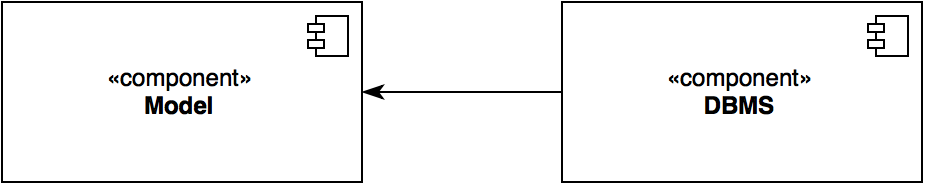
\includegraphics[scale=0.25]{seq1.png}
	}
\end{figure}

\textbf{Power Grid Stations Manager}
On the Resource Management Subsystem we can start from integrating the Power Grid Stations Manager with the DBMS.
The PGS Manager is almost fully independent from the other components and can be tested easily.
\begin{figure}[H]
	\centering
	\makebox[\textwidth][c]{
		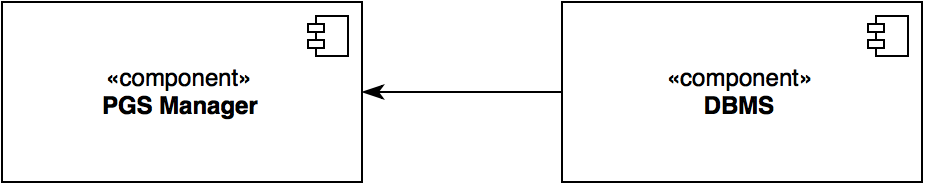
\includegraphics[scale=0.25]{seq2.png}
	}
\end{figure}

\paragraph{Car Handler}
The Car Handler is the component that is in charge of issuing commands to the car. We can start testing its behavior as soon as the Car Internal System is fully unit tested. We will make use of a stub to simulate the Resource Subsystem Interface.

\begin{figure}[H]
	\centering
	\makebox[\textwidth][c]{
		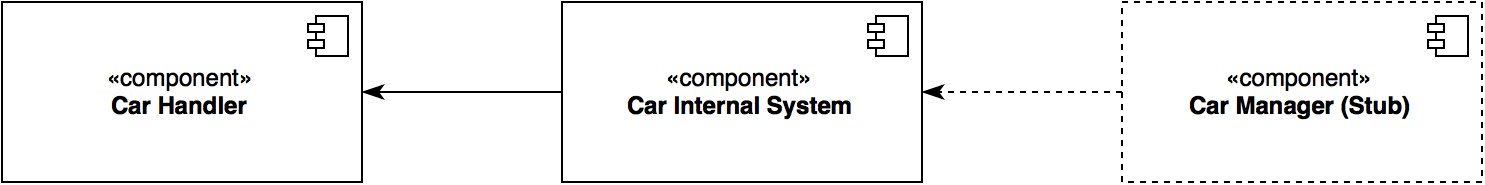
\includegraphics[scale=0.25]{seq3b.png}
	}
\end{figure}

\paragraph{Car Manager}
After the Car Handler is integrated we can finally incorporate the Car Manager, the component doing the heavy lifting in the Resource Management Subsystem.
\begin{figure}[H]
	\centering
	\makebox[\textwidth][c]{
		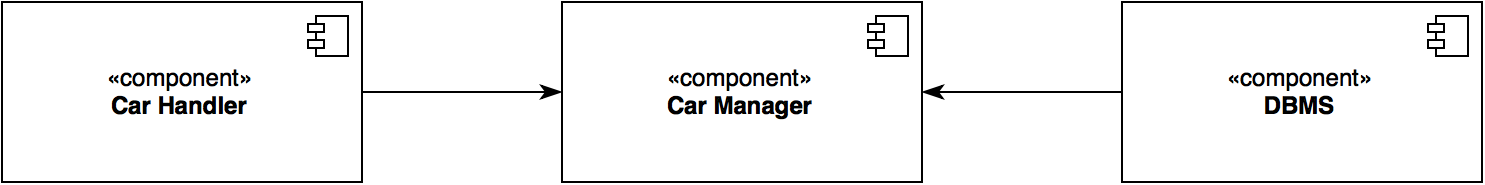
\includegraphics[scale=0.25]{seq4.png}
	}
\end{figure}

Once the Car Manager has been integration tested, we can actually test the interaction between the Car Internal System and the Resource Subsystem Interface.
\begin{figure}[H]
	\centering
	\makebox[\textwidth][c]{
		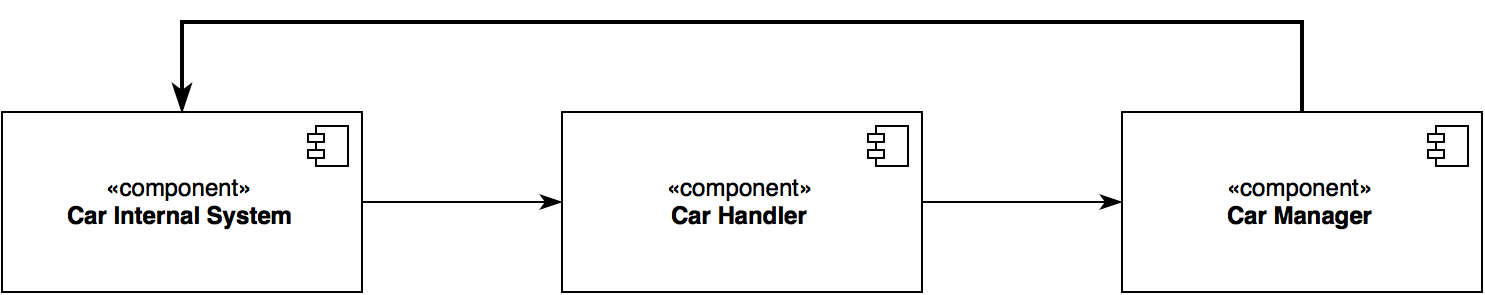
\includegraphics[scale=0.25]{seq-ciclo-a.png}
	}
\end{figure}

At this point the Resource Management Subsystem is fully integrated.
\begin{figure}[H]
	\centering
	\makebox[\textwidth][c]{
		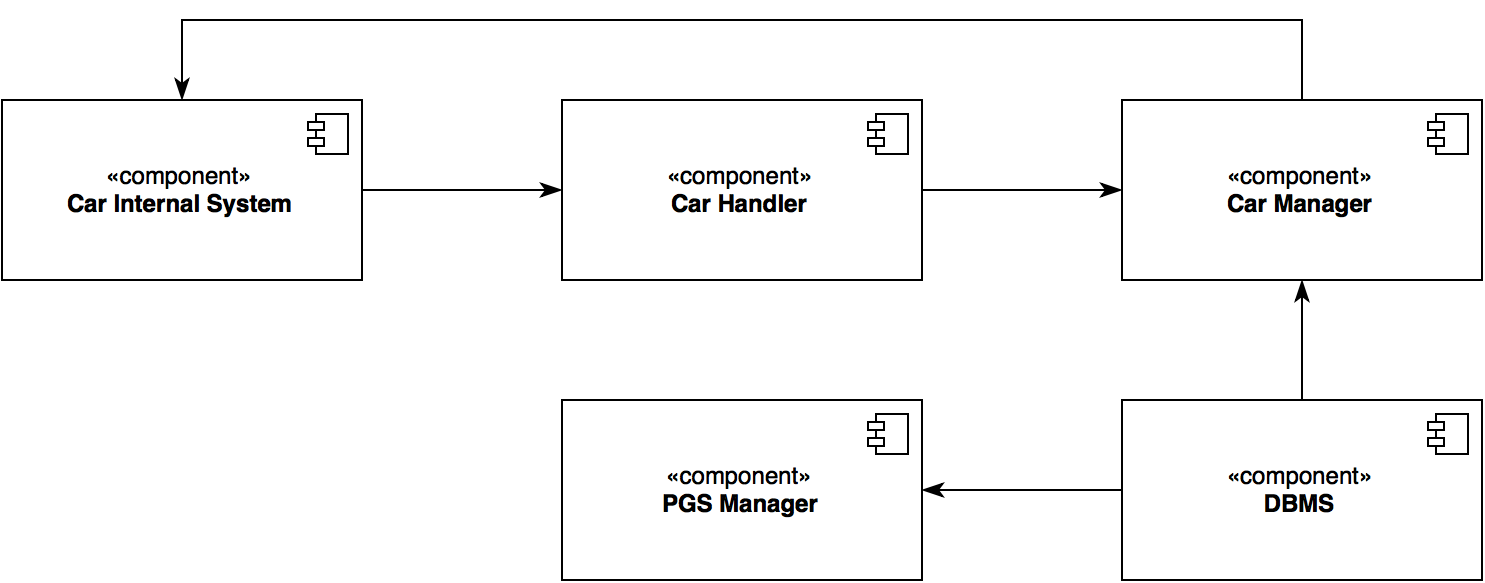
\includegraphics[scale=0.25]{seq-resource-subs.png}
	}
\end{figure}

\paragraph{Application and Resource Subsystems Integration}
We can now proceed to integrating the Application Subsystem and the Resource Subsystem, again following the bottom-up approach.
\begin{figure}[H]
	\centering
	\makebox[\textwidth][c]{
		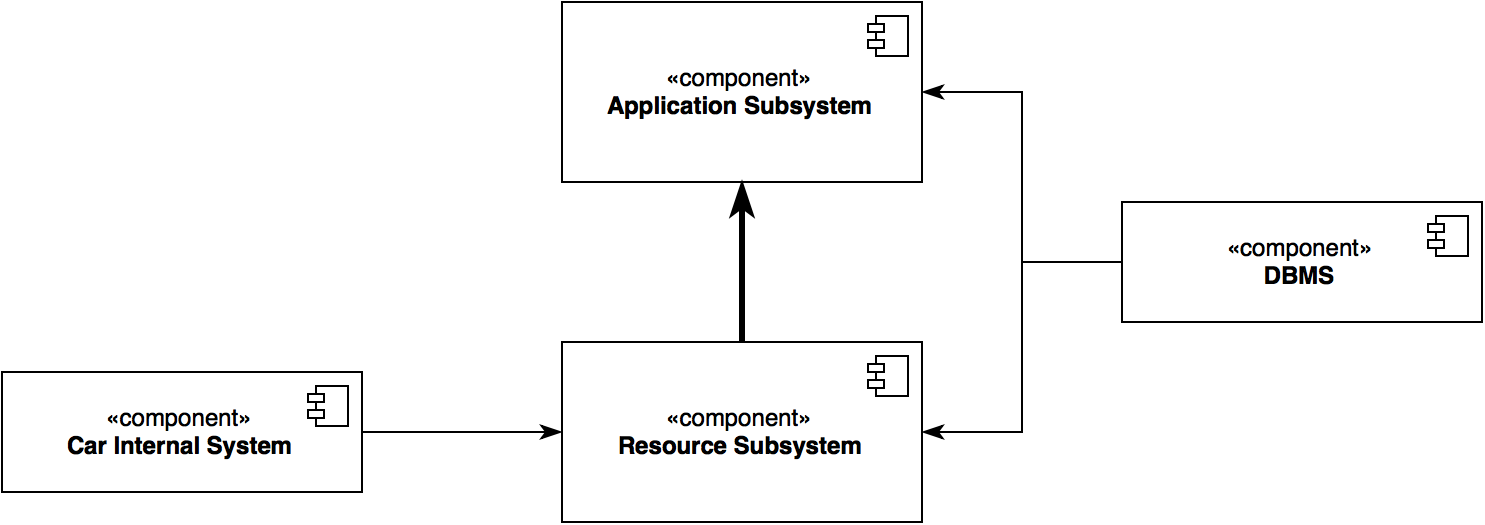
\includegraphics[scale=0.25]{seq-subsystemv1.png}
	}
\end{figure}

\paragraph{Application Subsystem Components}
Most of the components in the Application Subsystem are independent from each other, therefore they can be freely tested in parallel.

The Registration Component, the Account Manager, the Car Search Component, the PGS Search Component, the Safe Areas Search Component and the Payment Component only need the Model, while the Reservation Manager, the Unlocking Component, the Parking Component, the Ride Manager and the Report Manager also need to interface with the Resource Subsystem.



\begin{figure}[H]
	\centering
	\makebox[\textwidth][c]{
		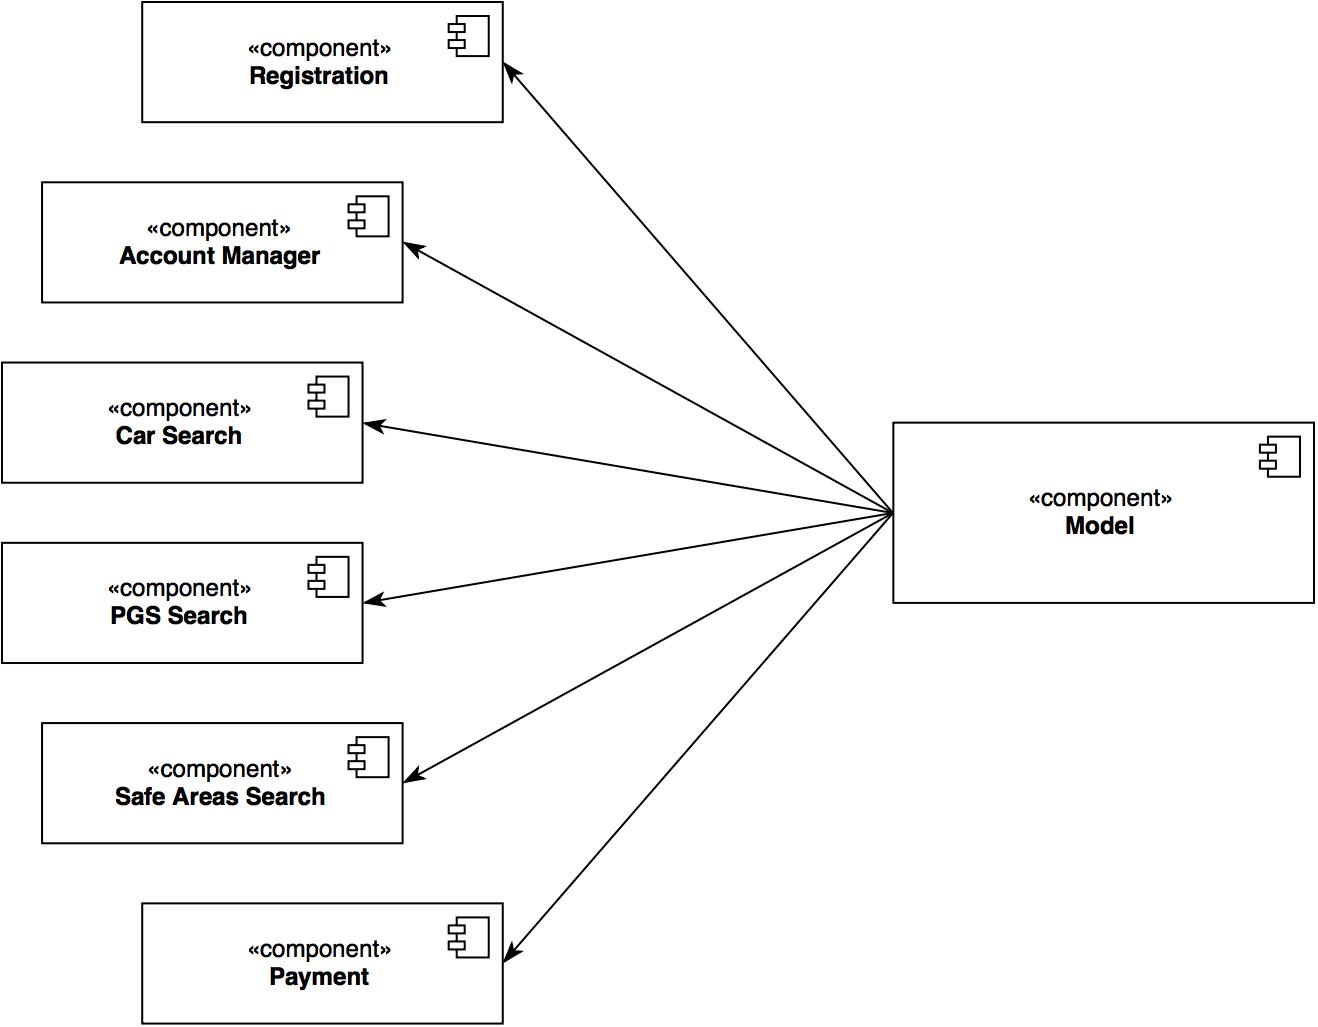
\includegraphics[scale=0.25]{seq-model1.png}
	}
\end{figure}
\begin{figure}[H]
	\centering
	\makebox[\textwidth][c]{
		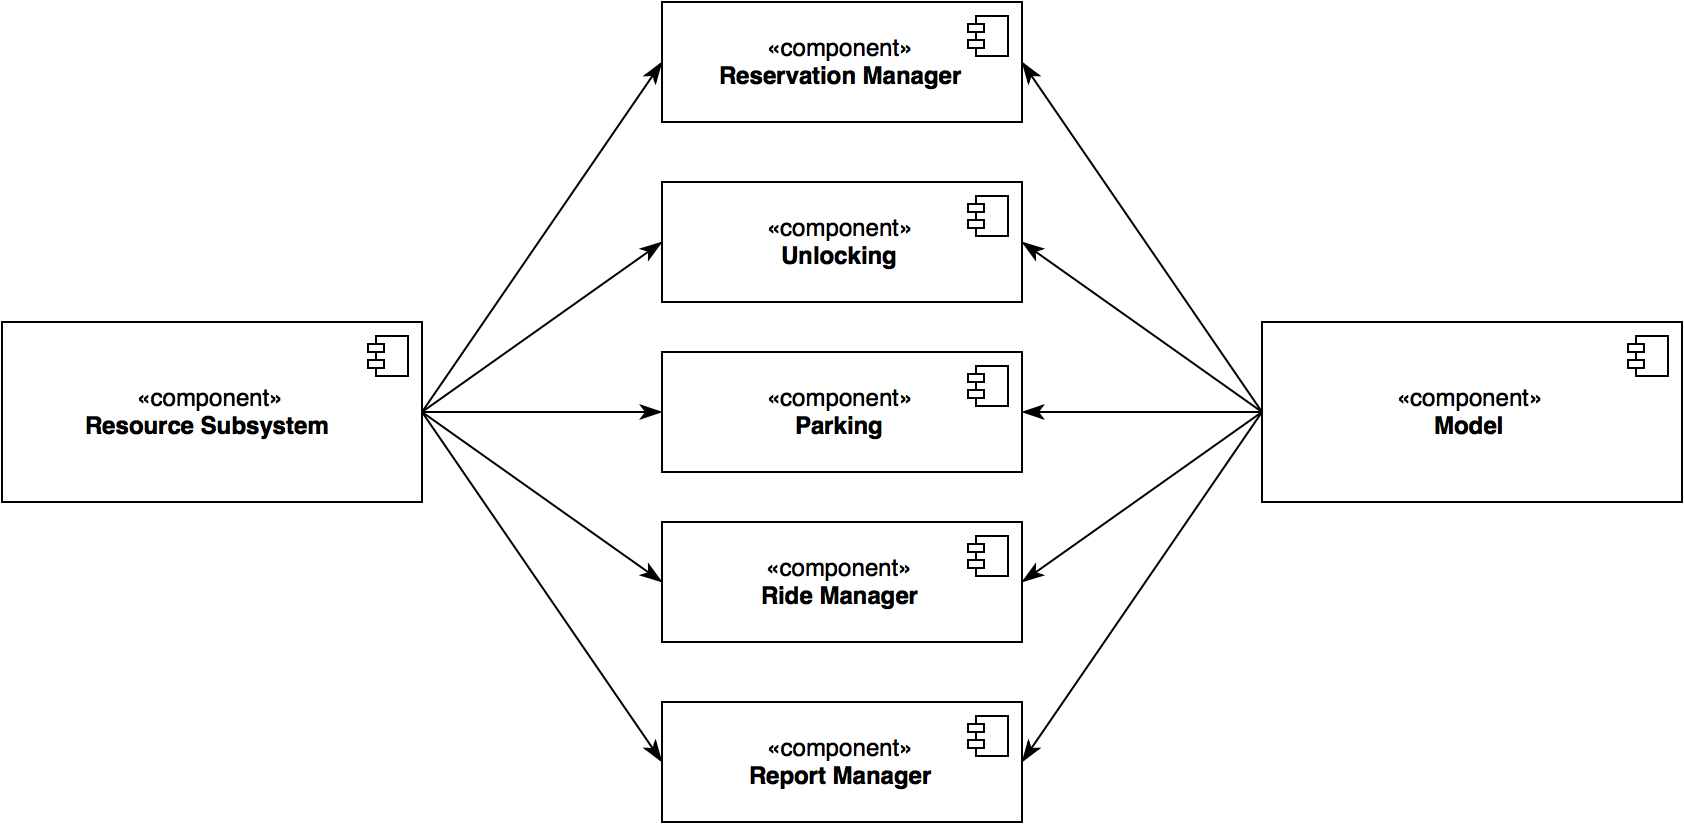
\includegraphics[scale=0.25]{seq-model2b.png}
	}
\end{figure}


\paragraph{Request Dispatcher}
The Request Dispatcher acts as a wrapper for all of the requests to the application API, processing and distributing them to the corresponding components.

This allows us to integrate it with thread based testing: when testing for one of the intermediate components has been finished, we can test the corresponding functionality on the Request Dispatcher, that will interact with the specific component.
The request dispatcher will be integrated one by one with all the other components, until the Application Subsystem is complete.

\begin{figure}[H]
	\centering
	\makebox[\textwidth][c]{
		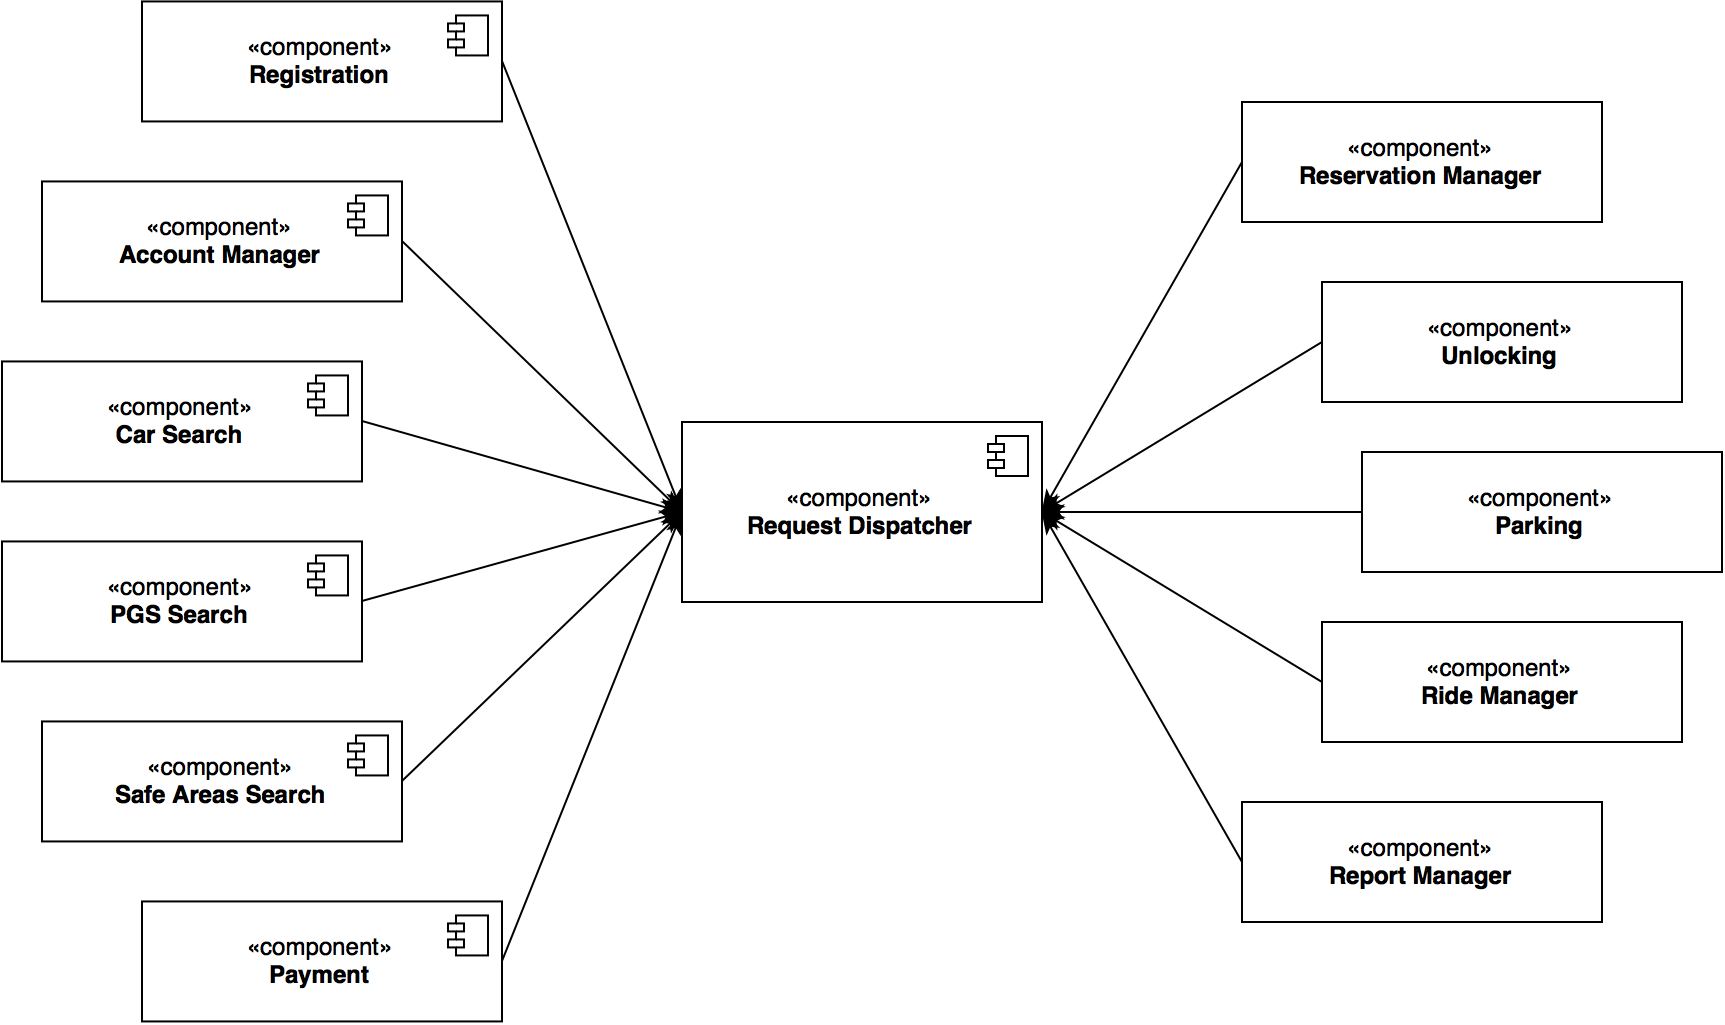
\includegraphics[scale=0.25]{seq-dispatcher.png}
	}
\end{figure}


\subsubsection{Client Applications Integration Sequence}
Finally, after the whole central system is tested and has been successfully integrated, we will test the interaction between the client applications and the system.

\begin{figure}[H]
	\centering
	\makebox[\textwidth][c]{
		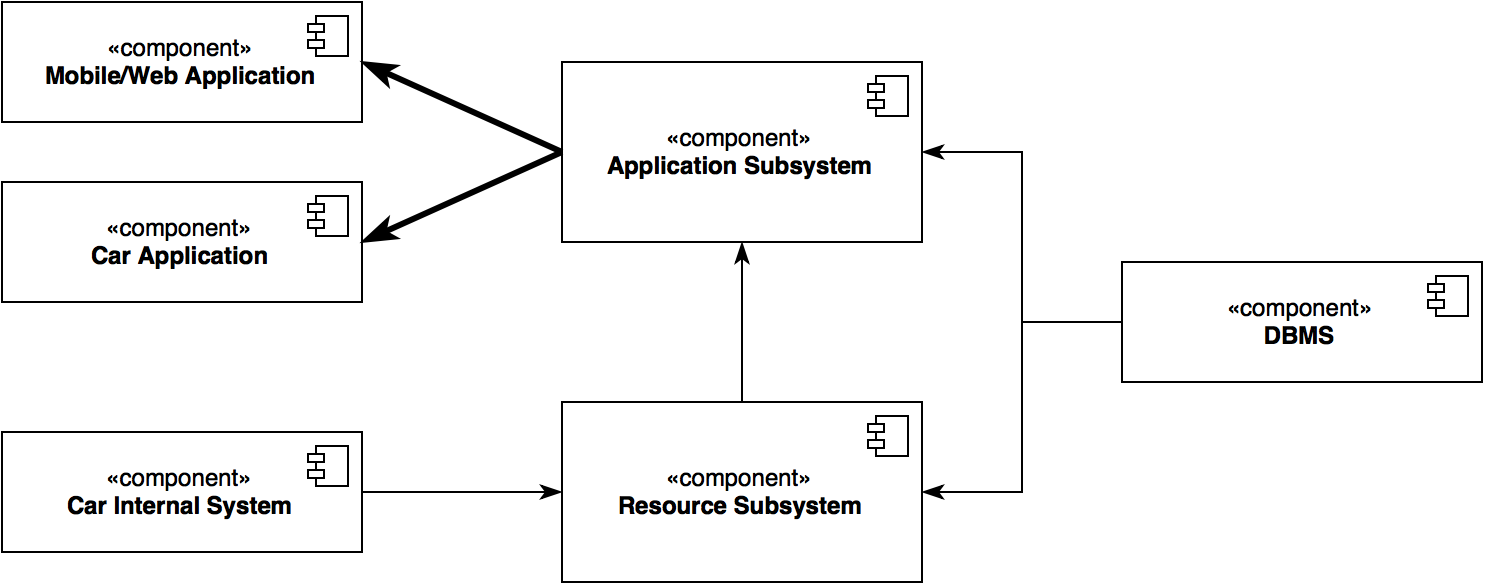
\includegraphics[scale=0.25]{seq-clients.png}
	}
\end{figure}



\section{Individual Steps and Test Description}

% qui se vogliamo potremmo dire che non descriviamo tutti i metodi esistenti ma solo quelli critici/più importanti

% Non serve scrivere metodi, basta dire cose come "Qui passiamo nomi utente e dati della patente, successo, poi passiamo nomi utente già esistenti, ci aspettiamo errore, poi patente errata, errore,..."

%TODO aggiungere tipi di input per ogni azione
%TODO aggiungere casi di input errati per ogni azione
%TODO aggiungere risultati per ognuno degli input
%TODO riscrivere tutto bene

\subsection{Model - DBMS}
azioni da componenti sul model
- le azioni di delete
- richieste di tutte le reservation/ride esistenti (serve?)
- select su tutti gli oggetti

% btw il model non fa check sulle cose inserite, tutti i controlli vengono effettuati a monte sui componenti dell'applicazione 

\begin{center}

	\begin{tabular}{ | p{6cm} | p{6cm} | }
		\hline 


		\hline

		\multicolumn{2}{|c|}{\textbf{Insert User}} \\
		\hline
		\multicolumn{1}{|c|}{\textit{Input}} & \multicolumn{1}{c|}{\textit{Result}} \\
		\hline
		A username, the user's personal data, an email and a payment method (e.g. a valid credit card number). & A new user is inserted in the database. \\
		\hline
		Some of the parameters are missing. & The insertion fails. \\
		\hline
		& \\
		\hline
	\end{tabular}
\end{center}
\begin{center}

	\begin{tabular}{ | p{6cm} | p{6cm} | }
		\hline 


		\hline

		\multicolumn{2}{|c|}{\textbf{Update User}} \\
		\hline
		\multicolumn{1}{|c|}{\textit{Input}} & \multicolumn{1}{c|}{\textit{Result}} \\
		\hline
		correct request & user data updated \\
		\hline
		updating with unacceptable data & fail \\
		\hline
		trying to update a nonexistent user & fail \\
		\hline
	\end{tabular}
\end{center}

\begin{center}

	\begin{tabular}{ | p{6cm} | p{6cm} | }
		\hline 


		\hline

		\multicolumn{2}{|c|}{\textbf{Insert Bill}} \\
		\hline
		\multicolumn{1}{|c|}{\textit{Input}} & \multicolumn{1}{c|}{\textit{Result}} \\
		\hline
		un utente valido e una bill ben formata & aggiunge la bill all'utente \\
		\hline
		un utente valido e una bill non ben formata & errore \\
		\hline
		un utente inesistente e una bill qualsiasi & errore \\
		\hline
	\end{tabular}
\end{center}

\begin{center}

	\begin{tabular}{ | p{6cm} | p{6cm} | }
		\hline 


		\hline

		\multicolumn{2}{|c|}{\textbf{List Bills}} \\
		\hline
		\multicolumn{1}{|c|}{\textit{Input}} & \multicolumn{1}{c|}{\textit{Result}} \\
		\hline
		un utente con bills & ritorna una lista di bills \\
		\hline
		un utente senza bills & ritorna una lista vuota \\
		\hline
		un utente inesistente & errore \\
		\hline
	\end{tabular}
\end{center}

\begin{center}

	\begin{tabular}{ | p{6cm} | p{6cm} | }
		\hline 


		\hline

		\multicolumn{2}{|c|}{\textbf{List Cars}} \\
		\hline
		\multicolumn{1}{|c|}{\textit{Input}} & \multicolumn{1}{c|}{\textit{Result}} \\
		\hline
		niente & lista di tutte le macchine e informazioni allegate \\
		\hline
	\end{tabular}
\end{center}

\begin{center}

	\begin{tabular}{ | p{6cm} | p{6cm} | }
		\hline 


		\hline

		\multicolumn{2}{|c|}{\textbf{List Power Grid Stations}} \\
		\hline
		\multicolumn{1}{|c|}{\textit{Input}} & \multicolumn{1}{c|}{\textit{Result}} \\
		\hline
		niente &  \\
		\hline
	\end{tabular}
\end{center}

\begin{center}

	\begin{tabular}{ | p{6cm} | p{6cm} | }
		\hline 


		\hline

		\multicolumn{2}{|c|}{\textbf{List Safe Areas}} \\
		\hline
		\multicolumn{1}{|c|}{\textit{Input}} & \multicolumn{1}{c|}{\textit{Result}} \\
		\hline
		input1 & result1 \\
		\hline
		input2 & result2 \\
		\hline
	\end{tabular}
\end{center}

\begin{center}

	\begin{tabular}{ | p{6cm} | p{6cm} | }
		\hline 


		\hline

		\multicolumn{2}{|c|}{\textbf{Insert Reservation}} \\
		\hline
		\multicolumn{1}{|c|}{\textit{Input}} & \multicolumn{1}{c|}{\textit{Result}} \\
		\hline
		input1 & result1 \\
		\hline
		input2 & result2 \\
		\hline
	\end{tabular}
\end{center}

\begin{center}

	\begin{tabular}{ | p{6cm} | p{6cm} | }
		\hline 


		\hline

		\multicolumn{2}{|c|}{\textbf{Update Reservation}} \\
		\hline
		\multicolumn{1}{|c|}{\textit{Input}} & \multicolumn{1}{c|}{\textit{Result}} \\
		\hline
		input1 & result1 \\
		\hline
		input2 & result2 \\
		\hline
	\end{tabular}
\end{center}

\begin{center}

	\begin{tabular}{ | p{6cm} | p{6cm} | }
		\hline 


		\hline

		\multicolumn{2}{|c|}{\textbf{Insert Ride}} \\
		\hline
		\multicolumn{1}{|c|}{\textit{Input}} & \multicolumn{1}{c|}{\textit{Result}} \\
		\hline
		input1 & result1 \\
		\hline
		input2 & result2 \\
		\hline
	\end{tabular}
\end{center}


\begin{center}

	\begin{tabular}{ | p{6cm} | p{6cm} | }
		\hline 


		\hline

		\multicolumn{2}{|c|}{\textbf{Update Ride}} \\
		\hline
		\multicolumn{1}{|c|}{\textit{Input}} & \multicolumn{1}{c|}{\textit{Result}} \\
		\hline
		input1 & result1 \\
		\hline
		input2 & result2 \\
		\hline
	\end{tabular}
\end{center}

\subsection{PGS Manager - DBMS}
azioni da interfaccia esterna
- update plugs
	-> disponibile
	-> non disponibile
in teoria non dovrebbero esserci richieste errate perché sono solo messaggi delle stazioni, ma mettiamo casi di errore

\begin{center}

	\begin{tabular}{ | p{6cm} | p{6cm} | }
		\hline 


		\hline

		\multicolumn{2}{|c|}{\textbf{Update Plug Availability}} \\
		\hline
		\multicolumn{1}{|c|}{\textit{Input}} & \multicolumn{1}{c|}{\textit{Result}} \\
		\hline
		input1 & result1 \\
		\hline
		input2 & result2 \\
		\hline
	\end{tabular}
\end{center}

\subsection{Car Handler - Car Internal System}
azioni da car manager a car handler
- richiesta di informazioni
- lock
- unlock

\begin{center}

	\begin{tabular}{ | p{6cm} | p{6cm} | }
		\hline 


		\hline

		\multicolumn{2}{|c|}{\textbf{Request Update from Car}} \\
		\hline
		\multicolumn{1}{|c|}{\textit{Input}} & \multicolumn{1}{c|}{\textit{Result}} \\
		\hline
		input1 & result1 \\
		\hline
		input2 & result2 \\
		\hline
	\end{tabular}
\end{center}

\begin{center}

	\begin{tabular}{ | p{6cm} | p{6cm} | }
		\hline 


		\hline

		\multicolumn{2}{|c|}{\textbf{Lock Car}} \\
		\hline
		\multicolumn{1}{|c|}{\textit{Input}} & \multicolumn{1}{c|}{\textit{Result}} \\
		\hline
		input1 & result1 \\
		\hline
		input2 & result2 \\
		\hline
	\end{tabular}
\end{center}

\begin{center}

	\begin{tabular}{ | p{6cm} | p{6cm} | }
		\hline 


		\hline

		\multicolumn{2}{|c|}{\textbf{Unlock Car}} \\
		\hline
		\multicolumn{1}{|c|}{\textit{Input}} & \multicolumn{1}{c|}{\textit{Result}} \\
		\hline
		input1 & result1 \\
		\hline
		input2 & result2 \\
		\hline
	\end{tabular}
\end{center}

\subsection{Car Manager - Car Handler - DBMS}
richieste da: maintenance, application subsystem, macchine
maintenance
- lista macchine
- set macchina available
- set macchina unavailable
application:
- lock
- unlock
macchina:
- aggiornamento informazioni (solite posizione, batteria ecc.)

\subsubsection{Maintenance}
\begin{center}

	\begin{tabular}{ | p{6cm} | p{6cm} | }
		\hline 


		\hline

		\multicolumn{2}{|c|}{\textbf{List Cars in Need of Maintenance}} \\
		\hline
		\multicolumn{1}{|c|}{\textit{Input}} & \multicolumn{1}{c|}{\textit{Result}} \\
		\hline
		input1 & result1 \\
		\hline
		input2 & result2 \\
		\hline
	\end{tabular}
\end{center}

\begin{center}

	\begin{tabular}{ | p{6cm} | p{6cm} | }
		\hline 


		\hline

		\multicolumn{2}{|c|}{\textbf{Set Car as Available}} \\
		\hline
		\multicolumn{1}{|c|}{\textit{Input}} & \multicolumn{1}{c|}{\textit{Result}} \\
		\hline
		input1 & result1 \\
		\hline
		input2 & result2 \\
		\hline
	\end{tabular}
\end{center}

\begin{center}

	\begin{tabular}{ | p{6cm} | p{6cm} | }
		\hline 


		\hline

		\multicolumn{2}{|c|}{\textbf{Set Car as Unavailable}} \\
		\hline
		\multicolumn{1}{|c|}{\textit{Input}} & \multicolumn{1}{c|}{\textit{Result}} \\
		\hline
		input1 & result1 \\
		\hline
		input2 & result2 \\
		\hline
	\end{tabular}
\end{center}

\subsubsection{Interface to the Application Subsystem}
\begin{center}

	\begin{tabular}{ | p{6cm} | p{6cm} | }
		\hline 


		\hline

		\multicolumn{2}{|c|}{\textbf{Request to Lock Car}} \\
		\hline
		\multicolumn{1}{|c|}{\textit{Input}} & \multicolumn{1}{c|}{\textit{Result}} \\
		\hline
		input1 & result1 \\
		\hline
		input2 & result2 \\
		\hline
	\end{tabular}
\end{center}

\begin{center}

	\begin{tabular}{ | p{6cm} | p{6cm} | }
		\hline 


		\hline

		\multicolumn{2}{|c|}{\textbf{Request to Unlock Car}} \\
		\hline
		\multicolumn{1}{|c|}{\textit{Input}} & \multicolumn{1}{c|}{\textit{Result}} \\
		\hline
		input1 & result1 \\
		\hline
		input2 & result2 \\
		\hline
	\end{tabular}
\end{center}

\subsubsection{Car Interface}
\begin{center}

	\begin{tabular}{ | p{6cm} | p{6cm} | }
		\hline 


		\hline

		\multicolumn{2}{|c|}{\textbf{Car Status Update}} \\
		\hline
		\multicolumn{1}{|c|}{\textit{Input}} & \multicolumn{1}{c|}{\textit{Result}} \\
		\hline
		input1 & result1 \\
		\hline
		input2 & result2 \\
		\hline
	\end{tabular}
\end{center}

\subsection{Application Subsystem Components - Model}
azioni da request dispatcher


\subsubsection{Registration Component - Model}
- registrazione utente
\begin{center}

	\begin{tabular}{ | p{6cm} | p{6cm} | }
		\hline 


		\hline

		\multicolumn{2}{|c|}{\textbf{Register User}} \\
		\hline
		\multicolumn{1}{|c|}{\textit{Input}} & \multicolumn{1}{c|}{\textit{Result}} \\
		\hline
		input1 & result1 \\
		\hline
		input2 & result2 \\
		\hline
	\end{tabular}
\end{center}

\subsubsection{Account Manager - Model}
- login
- getinfo utente
- update info utente
- list bills
\begin{center}

	\begin{tabular}{ | p{6cm} | p{6cm} | }
		\hline 


		\hline

		\multicolumn{2}{|c|}{\textbf{Login}} \\
		\hline
		\multicolumn{1}{|c|}{\textit{Input}} & \multicolumn{1}{c|}{\textit{Result}} \\
		\hline
		input1 & result1 \\
		\hline
		input2 & result2 \\
		\hline
	\end{tabular}
\end{center}

\begin{center}

	\begin{tabular}{ | p{6cm} | p{6cm} | }
		\hline 


		\hline

		\multicolumn{2}{|c|}{\textbf{Get User Info}} \\
		\hline
		\multicolumn{1}{|c|}{\textit{Input}} & \multicolumn{1}{c|}{\textit{Result}} \\
		\hline
		input1 & result1 \\
		\hline
		input2 & result2 \\
		\hline
	\end{tabular}
\end{center}

\begin{center}

	\begin{tabular}{ | p{6cm} | p{6cm} | }
		\hline 


		\hline

		\multicolumn{2}{|c|}{\textbf{Update User Info}} \\
		\hline
		\multicolumn{1}{|c|}{\textit{Input}} & \multicolumn{1}{c|}{\textit{Result}} \\
		\hline
		input1 & result1 \\
		\hline
		input2 & result2 \\
		\hline
	\end{tabular}
\end{center}

\begin{center}

	\begin{tabular}{ | p{6cm} | p{6cm} | }
		\hline 


		\hline

		\multicolumn{2}{|c|}{\textbf{List User Bills}} \\
		\hline
		\multicolumn{1}{|c|}{\textit{Input}} & \multicolumn{1}{c|}{\textit{Result}} \\
		\hline
		input1 & result1 \\
		\hline
		input2 & result2 \\
		\hline
	\end{tabular}
\end{center}

\subsubsection{Car Search Component- Model}
- find cars with position
- find cars with address

\begin{center}

	\begin{tabular}{ | p{6cm} | p{6cm} | }
		\hline 


		\hline

		\multicolumn{2}{|c|}{\textbf{Find Cars with Position}} \\
		\hline
		\multicolumn{1}{|c|}{\textit{Input}} & \multicolumn{1}{c|}{\textit{Result}} \\
		\hline
		input1 & result1 \\
		\hline
		input2 & result2 \\
		\hline
	\end{tabular}
\end{center}

\begin{center}

	\begin{tabular}{ | p{6cm} | p{6cm} | }
		\hline 


		\hline

		\multicolumn{2}{|c|}{\textbf{Find Cars with Address}} \\
		\hline
		\multicolumn{1}{|c|}{\textit{Input}} & \multicolumn{1}{c|}{\textit{Result}} \\
		\hline
		input1 & result1 \\
		\hline
		input2 & result2 \\
		\hline
	\end{tabular}
\end{center}

\subsubsection{PGS Search Component- Model}
- find stations with position
- find stations with address

\begin{center}

	\begin{tabular}{ | p{6cm} | p{6cm} | }
		\hline 


		\hline

		\multicolumn{2}{|c|}{\textbf{Find Stations with Address}} \\
		\hline
		\multicolumn{1}{|c|}{\textit{Input}} & \multicolumn{1}{c|}{\textit{Result}} \\
		\hline
		input1 & result1 \\
		\hline
		input2 & result2 \\
		\hline
	\end{tabular}
\end{center}

\begin{center}

	\begin{tabular}{ | p{6cm} | p{6cm} | }
		\hline 


		\hline

		\multicolumn{2}{|c|}{\textbf{Find Stations with Position}} \\
		\hline
		\multicolumn{1}{|c|}{\textit{Input}} & \multicolumn{1}{c|}{\textit{Result}} \\
		\hline
		input1 & result1 \\
		\hline
		input2 & result2 \\
		\hline
	\end{tabular}
\end{center}

\subsubsection{Safe Areas Search Component - Model}
- find safe areas with position
- find safe areas with address

\begin{center}

	\begin{tabular}{ | p{6cm} | p{6cm} | }
		\hline 


		\hline

		\multicolumn{2}{|c|}{\textbf{Find Safe Areas with Position}} \\
		\hline
		\multicolumn{1}{|c|}{\textit{Input}} & \multicolumn{1}{c|}{\textit{Result}} \\
		\hline
		input1 & result1 \\
		\hline
		input2 & result2 \\
		\hline
	\end{tabular}
\end{center}

\begin{center}

	\begin{tabular}{ | p{6cm} | p{6cm} | }
		\hline 


		\hline

		\multicolumn{2}{|c|}{\textbf{Find Safe Areas with Address}} \\
		\hline
		\multicolumn{1}{|c|}{\textit{Input}} & \multicolumn{1}{c|}{\textit{Result}} \\
		\hline
		input1 & result1 \\
		\hline
		input2 & result2 \\
		\hline
	\end{tabular}
\end{center}

\subsubsection{Payment Component- Model}
- pay a bill 

\begin{center}

	\begin{tabular}{ | p{6cm} | p{6cm} | }
		\hline 


		\hline

		\multicolumn{2}{|c|}{\textbf{Pay a Bill}} \\
		\hline
		\multicolumn{1}{|c|}{\textit{Input}} & \multicolumn{1}{c|}{\textit{Result}} \\
		\hline
		input1 & result1 \\
		\hline
		input2 & result2 \\
		\hline
	\end{tabular}
\end{center}

\subsubsection{Reservation Manager - Model - Resource Subsystem}
- crea reservation
- annulla reservation

\begin{center}

	\begin{tabular}{ | p{6cm} | p{6cm} | }
		\hline 


		\hline

		\multicolumn{2}{|c|}{\textbf{Create Reservation}} \\
		\hline
		\multicolumn{1}{|c|}{\textit{Input}} & \multicolumn{1}{c|}{\textit{Result}} \\
		\hline
		input1 & result1 \\
		\hline
		input2 & result2 \\
		\hline
	\end{tabular}
\end{center}

\begin{center}

	\begin{tabular}{ | p{6cm} | p{6cm} | }
		\hline 


		\hline

		\multicolumn{2}{|c|}{\textbf{Cancel Reservation}} \\
		\hline
		\multicolumn{1}{|c|}{\textit{Input}} & \multicolumn{1}{c|}{\textit{Result}} \\
		\hline
		input1 & result1 \\
		\hline
		input2 & result2 \\
		\hline
	\end{tabular}
\end{center}

\subsubsection{Unlocking Component - Model - Resource Subsystem}
- sblocca macchina (-> nb fa partire il conto del tempo)

ricordarsi che serve la posizione dell'utente vicina alla macchina!

\begin{center}

	\begin{tabular}{ | p{6cm} | p{6cm} | }
		\hline 


		\hline

		\multicolumn{2}{|c|}{\textbf{Unlock Car from Application}} \\
		\hline
		\multicolumn{1}{|c|}{\textit{Input}} & \multicolumn{1}{c|}{\textit{Result}} \\
		\hline
		input1 & result1 \\
		\hline
		input2 & result2 \\
		\hline
	\end{tabular}
\end{center}

\subsubsection{Parking Component - Model - Resource Subsystem}
- metti la macchina in sosta

\begin{center}

	\begin{tabular}{ | p{6cm} | p{6cm} | }
		\hline 


		\hline

		\multicolumn{2}{|c|}{\textbf{Park Car}} \\
		\hline
		\multicolumn{1}{|c|}{\textit{Input}} & \multicolumn{1}{c|}{\textit{Result}} \\
		\hline
		input1 & result1 \\
		\hline
		input2 & result2 \\
		\hline
	\end{tabular}
\end{center}

\subsubsection{Ride Manager - Model - Resource Subsystem}
- fine ride

\begin{center}

	\begin{tabular}{ | p{6cm} | p{6cm} | }
		\hline 


		\hline

		\multicolumn{2}{|c|}{\textbf{End Ride}} \\
		\hline
		\multicolumn{1}{|c|}{\textit{Input}} & \multicolumn{1}{c|}{\textit{Result}} \\
		\hline
		input1 & result1 \\
		\hline
		input2 & result2 \\
		\hline
	\end{tabular}
\end{center}

\subsubsection{Report Manager - Model - Resource Subsystem}
- aggiungi report

\begin{center}

	\begin{tabular}{ | p{6cm} | p{6cm} | }
		\hline 


		\hline

		\multicolumn{2}{|c|}{\textbf{Report Issue}} \\
		\hline
		\multicolumn{1}{|c|}{\textit{Input}} & \multicolumn{1}{c|}{\textit{Result}} \\
		\hline
		input1 & result1 \\
		\hline
		input2 & result2 \\
		\hline
	\end{tabular}
\end{center}

request dispatcher:
\subsection{Request Dispatcher - Application Components}
- questa è l'api descritta nel DD, diciamo soltanto che deve comportarsi nel modo che abbiamo già detto nei dettagli

client applications:
\subsection{Mobile/Web Application - Application Subsystem}
- qui diciamo che proviamo l'applicazione in tutte le sue funzionalità e devono funzionare tutte

\subsection{Car Application - Application Subsystem}
- stessa cosa qui

%% se necessario possiamo usare longtable
\begin{center}

	\begin{tabular}{ | p{6cm} | p{6cm} | }
		\hline 


		\hline

		\multicolumn{2}{|c|}{\textbf{method(arg1, arg2)}} \\
		\hline
		\multicolumn{1}{|c|}{\textit{Input}} & \multicolumn{1}{c|}{\textit{Result}} \\
		\hline
		input1 & result1 \\
		\hline
		input2 & result2 \\
		\hline
	\end{tabular}
\end{center}

\section{Tools and Test Equipment Required}

\section{Program Stubs and Test Data Required}

\subsection{Program Stubs and Drivers}

\subsection{Test Data}

For the sake of completeness, the data used in the tests allow us to verify the proper behavior and the reaction to any kind of incorrect practice. Moreover the DB will be populated with appropriate data to perform the tests.
In furtherance of accomplish the necessary tests, we are going to need:

\begin{itemize}
  \item{A list of both valid and invalid sign up data to test the \textbf{Registration} component.
  The collection of data should contain instances exhibiting the following problems: (copiata)
    \begin{itemize}
      \item{Correct biographical data}
      \item{Biographical data with numeric characters and notation}
      \item{DOB compliant with the ISDTN UNI EN 28601} (meticolosità a non finire)
      \item{DOB \underline{not} compliant with the ISDTN UNI EN 28601}
      \item{Not existent email address}
      \item{Valid email address}
      \item{Valid driving license}
      \item{Suspended driving license}
      \item{Not existing driving license}
      \item{Driving license \underline{not} compliant with legal format}
      \item{Valid credit card number}
      \item{Credit card number \underline{not} compliant with legal format}
      \item{Valid credit card CVV}
      \item{\underline{Not} valid credit card CVV}
    \end{itemize}}

    \item{A list of both valid and invalid \textbf{non ho idea di cosa mettere} to test the \textbf{Account Manager} component.
    The collection of data should contain instances exhibiting the following problems:
    \begin{itemize}
      \item{Valid username}
      \item{Not existing username}
      \item{Valid password}
      \item{\underline{Not} valid password}
    \end{itemize}}

    \item{A list of both valid and invalid tracing data to test the \textbf{Car Search} component.
    The collection of data should contain instances exhibiting the following problems:
    \begin{itemize}
      \item{Valid position}
      \item{\underline{Not} existing position}
      \item{Position outside safe areas}
      \item{Valid address}
      \item{\underline{Not} valid address}
      \item{\underline{Not} existing address}
      \item{Address outside safe areas}
    \end{itemize}}

    \item{A list of both valid and invalid tracing data to test the \textbf{PGS Search} component.
    The collection of data should contain instances exhibiting the following problems:
    \begin{itemize}
      \item{Valid position}
      \item{\underline{Not} existing position}
      \item{Position outside safe areas}
      \item{Valid address}
      \item{\underline{Not} valid address}
      \item{\underline{Not} existing address}
      \item{Address outside safe areas}
    \end{itemize}}

    \item{A list of both valid and invalid tracing data to test the \textbf{Safe Areas Search} component.
    The collection of data should contain instances exhibiting the following problems:
    \begin{itemize}
      \item{Valid position}
      \item{\underline{Not} existing position}
      \item{Position outside safe areas}
      \item{Valid address}
      \item{\underline{Not} valid address}
      \item{\underline{Not} existing address}
      \item{Address outside safe areas}
    \end{itemize}}

    \item{A list of both valid and invalid banking data to test the \textbf{Payment} component.
    The collection of data should contain instances exhibiting the following problems:
    \begin{itemize}
      \item{Valid credit card number}
      \item{Credit card number \underline{not} compliant with legal format}
      \item{Valid credit card CVV}
      \item{\underline{Not} valid credit card CVV}
    \end{itemize}}

    \item{A list of both valid and invalid user data to test the \textbf{Reservation Management} component.
    The collection of data should contain instances exhibiting the following problems:
    \begin{itemize}
      \item{Valid username}
      \item{Not existing username}
      \item{Valid password}
      \item{\underline{Not} valid password}
      \item{List of cars on DB}
    \end{itemize}}

    \item{A list of both valid and invalid user and tracing data to test the \textbf{Unlock} component.
    The collection of data should contain instances exhibiting the following problems:
    \begin{itemize}
      \item{Valid username}
      \item{Not existing username}
      \item{Valid password}
      \item{\underline{Not} valid password}
      \item{Valid position}
      \item{\underline{Not} existing position}
      \item{Position outside safe areas}
      \item{Valid QR Code}
      \item{\underline{Not} valid QR Code}
      \item{List of cars on DB}
    \end{itemize}}

    \item{A list of both valid and invalid user and tracing data to test the \textbf{Ride} component.
    The collection of data should contain instances exhibiting the following problems:
    \begin{itemize}
      \item{Valid username}
      \item{Not existing username}
      \item{Valid password}
      \item{\underline{Not} valid password}
      \item{Valid position}
      \item{\underline{Not} existing position}
      \item{Position outside safe areas}
    \end{itemize}}

    \item{A list of both valid and invalid user data to test the \textbf{Report Manager} component.
    The collection of data should contain instances exhibiting the following problems:
    \begin{itemize}
      \item{Valid username}
      \item{Not existing username}
      \item{Valid password}
      \item{\underline{Not} valid password}
      \item{Valid input field for the form}
      \item{Null input field for the form}
      \item{List of cars on DB}
    \end{itemize}}

\end{itemize}

\section{Effort Spent}
\begin{itemize}
	\item{Pietro Ferretti:  hours of work}
	\item{Nicole Gervasoni:  hours of work}
	\item{Danilo Labanca:  hours of work}
\end{itemize}

\end{document}
